\chapter{A Conceptual Model of Disturbances and Reliability Concerns in SoTS}
\label{ch:reliable-sots}
In SoS contexts, reliability is commonly understood as the ability to maintain operation despite \textbf{disturbances} arising from the dynamic behaviour of constituent systems~\cite{ferreira2023towards}. Disturbances may occur when systems join or leave the SoS, or when participating systems experience faults or produce incorrect behaviour. Such disturbances may \textbf{lead to unreliable} SoS---and by extension, unreliable SoTS (\secref{sec:disturbances-to-unreliability}). To reason about reliability in SoTS, disturbances must first be characterized. This chapter introduces a \textbf{conceptual characterization of disturbances} through two largely independent, but partially interacting, dimensions of constituent state: \emph{belonging} and \emph{health} (\secref{sec:two-dimensional-disturbances}). Building on this characterization, disturbances are then \textbf{analyzed using a state-based model} of constituent behaviour (\secref{sec:structured-reasoning}). The model is implemented using Statecharts \cite{harel1987statecharts} (\secref{sec:statecharts-reliability}). Using this representation, the chapter introduces a hierarchy of reliability levels that progressively restrict disturbance-causing configurations (\secref{sec:reliability-levels}). It then discusses how architectural reliability constraints reduce the burden on service-level fault tolerance (\secref{sec:reducing-fault-tolerance-burden}). Finally, the chapter examines how the proposed reliability levels align with different SoTS architectural types (\secref{sec:reliability-compatibility}).

% ==============================================================
\section{From Disturbances to (Un)Reliability in SoTS}\label{sec:disturbances-to-unreliability}

SoS differ from traditional engineered systems due to the operational and managerial independence of their constituent systems and their dynamically evolving configurations \cite{maier1998architecting}. Because constituents retain control over their own operation while contributing to a broader system mission, participants may join, leave, or modify their behaviour during operation. These dynamics complicate reasoning about how system-level behaviour can be maintained.

In the SoS reliability literature, events that disrupt coordinated behaviour are commonly described as \emph{disturbances}. \citet{ferreira2023towards} define a disturbance as any structural or operational change that negatively affects the ability of a constituent system, or the SoS as a whole, to deliver capabilities required for mission fulfilment. Disturbances may arise from changes in participation, reductions in system performance or availability, or faults within individual systems \cite{ferreira2023towards}. Because SoS capabilities depend on cooperation among interdependent constituents, such disturbances may propagate through the system and affect mission-level behaviour \cite{avizienis2004basic,li2025reliability}.

Observations from the SoTS literature reflect similar patterns. Disturbances frequently arise from changes in system participation, such as intermittent connectivity or the dynamic addition and removal of subsystems \cite{parri2019jarvis,human2023design,howard2021greenhouse}. Others originate from degraded operational behaviour, including missing data, delayed communication, or noisy sensor observations \cite{esterle2021digital,gill2022method,chen2018digital,duan2023digital}. These observations suggest that disturbances in SoTS commonly manifest through two forms of change: variations in constituent participation and variations in their operational health.

\begin{runningexample}{Disturbances in the CEP-Based SoTS}

The running CEP-based SoTS example illustrates these forms of disturbance.

\begin{center}
\begin{tikzpicture}[
    font=\footnotesize,
    twin/.style={
        rectangle, draw, rounded corners,
        minimum width=2.25cm,
        minimum height=0.9cm,
        inner ysep=2.5pt,
        fill=white,
        align=center
    },
    affected/.style={
        rectangle, draw=red, thick, rounded corners,
        minimum width=2.25cm,
        minimum height=0.9cm,
        inner ysep=2.5pt,
        fill=white,
        align=center
    },
    failed/.style={
        rectangle, draw=red, fill=red!20, thick,
        rounded corners,
        minimum width=2.25cm,
        minimum height=0.9cm,
        inner ysep=2.5pt,
        align=center
    },
    partially/.style={
        rectangle, draw=red, thick,
        rounded corners,
        minimum width=2.25cm,
        minimum height=0.9cm,
        inner ysep=2.5pt,
        fill=white,
        align=center
    },
    faded/.style={opacity=0.35},
    dependency/.style={gray!60, thin},
    disturbance/.style={red, very thick},
    disturbance_partial/.style={red, dashed, very thick},
    cep/.style={
        rectangle,
        draw,
        thick,
        fill=white,
        minimum width=4.35cm,
        align=center
    }
]

% DT1 after leaving
\node[twin] (dt1_out) at (-4.6,3.0) {DT$_1$};

% SoTS Boundary
\node[
    draw=black!60,
    thick,
    fill=white,
    rounded corners,
    minimum width=9.8cm,
    minimum height=4.1cm,
    label=above:{\textbf{SoTS}}
] (sos) at (0,0) {};

% Participating DTs
\node[twin,faded] (dt1) at (-2.9,0.85) {DT$_1$};

\node[failed]   (dt2) at (0,1.1)  {DT$_2$};
\node[affected] (dt3) at (2.9,0.85)  {DT$_3$};

\node[partially] (dt4) at (-1.45,-1.0) {DT$_4$};
\node[partially] (dt5) at (1.45,-1.0)  {DT$_5$};

% Interdependencies
\draw[dependency] (dt2) -- (dt3);
\draw[dependency] (dt3) -- (dt5);

% weakened dependency
\draw[gray!80, thin, dashed, ->] (dt1) -- (dt4);

% Disturbance propagation
\draw[disturbance, ->] (dt2) -- (dt3);
\draw[disturbance, ->] (dt3) -- (dt5);

% Leave transition
\draw[->, thick]
(dt1) to[out=115,in=-95]
node[left, font=\scriptsize, black!90]{left}
(dt1_out);

% CEP Layer
\node[cep, below=-0.12cm of sos.south] (cep)
{Complex Event Processing (CEP) Layer};

\end{tikzpicture}

\vspace{-4pt}
{\footnotesize Disturbance propagation within a SoTS:
\textcolor{red}{\(\rightarrow\)} propagation,
\tikz{\draw[red, thick, fill=red!20] (0,0) rectangle (0.25,0.25);} faulty DT,
\tikz{\draw[red, thick] (0,0) rectangle (0.25,0.25);} affected DT}
\end{center}

\begin{itemize}[noitemsep]
\item A DT leaves unexpectedly, removing observations required for global event detection and affecting dependent systems.
\item A degraded DT emits missing, delayed, or noisy events, introducing bias and uncertainty into system-level reasoning.
\end{itemize}

\end{runningexample}

In dependability theory, reliability is commonly defined as the continuity of correct service over time \cite{avizienis2004basic}. While classical dependability models provide a strong foundation for reasoning about reliability in engineered systems, SoTS introduce additional complexities due to evolving configurations and autonomous constituent behaviour. Reliability in SoTS can therefore be understood as the ability of the system to maintain operations despite disturbances affecting its constituent systems \cite{ferreira2023towards}. Understanding how such disturbances arise and propagate is essential for reasoning about reliability in SoTS. The following section introduces a conceptual model that represents these disturbances through two interacting dimensions of constituent state.

% ---
\section{A Two-Dimensional Disturbance Model for SoTS}
\label{sec:two-dimensional-disturbances}

Disturbances in SoTS can be understood through two observable aspects of constituent systems: whether they participate in the SoTS and whether they operate correctly while participating. I therefore model disturbances along two orthogonal dimensions: \emph{belonging}, which captures participation in the SoTS, and \emph{health}, which captures the operational condition of participating constituents.

Previous research has largely examined these aspects separately. Work on SoS structure and lifecycle focuses on how systems join, integrate with, or withdraw from the SoS \cite{axelsson2019refined,svenson2020situation,hristozov2023modeling}. In contrast, SoS reliability research studies how systems maintain operations despite faults and operational disturbances \cite{ferreira2024framework,uday2015designing,garro2014reliability,li2025reliability}.

In SoTS environments, however, participation and operational condition interact during system operation. Degradation in a constituent system may reduce its ability to contribute capabilities and, if persistent, may ultimately lead to the loss of that capability. In such cases, degradation in operational health can effectively result in a change in participation. Representing disturbances along these two dimensions allows participation and operational condition to be analysed independently while revealing how they interact during system operation. \tabref{tab:belonging-health} summarizes the possible combinations of belonging and health for a constituent system.


\begin{center}
\footnotesize
\begin{tabular}{p{2.5cm}|p{6cm}|p{6cm}}
& \textbf{Healthy} & \textbf{Unhealthy} \\
\hline
\textbf{Belongs}
& \textbf{Stable participation.} 
\newline Capabilities are available and effectively delivered, supporting mission fulfilment without introducing disturbance.
& \textbf{Degraded participation.} 
\newline Capabilities are available but delivered below expected performance, introducing operational disturbances that may influence dependent constituents. \\

\textbf{Does not belong}
& \textbf{Structural withdrawal.} 
\newline Operationally capable but structurally absent; its departure may disrupt dependent constituents and alter mission performance.
& \textbf{Externalized disturbance.} 
\newline Structurally absent and operationally impaired; instability originates outside the SoTS but may affect it upon re-entry. \\
\end{tabular}
\end{center}

In SoTS, capabilities emerge from the coordinated behaviour of loosely coupled and interdependent constituent systems. Because system-level capabilities depend on this coordination, disturbances affecting individual constituents may propagate and disrupt dependent systems. Constituent systems retain autonomy and may freely decide whether to join or leave the system \cite{boardman2006system,baldwin2011formation}. As observed by \citet{salado2015abandonment}, this autonomy naturally leads to situations where systems withdraw from participation, potentially destabilizing the SoTS by removing capabilities required for system operation \cite{salado2016exile}. Even while participating in the SoTS, impairments may cause a system to behave incorrectly or deliver reduced performance \cite{abbott1990resourceful}. Such faults may also propagate to dependent systems and affect their ability to deliver capabilities \cite{ferreira2024framework,avizienis2004basic}. In this context, \emph{belonging} captures whether a system participates in the SoTS and contributes capabilities, while \emph{health} captures whether participating systems deliver those capabilities correctly during operation.


\begin{runningexample}{Interaction Between Belonging and Health in a CEP-Based SoTS}
Consider the CEP-based SoTS introduced earlier. Suppose a constituent DT begins producing noisy observations due to degraded sensing capabilities. If this degradation persists, other systems may ignore its observations or the DT may be removed from the SoTS. In this case, degradation in the DT's \emph{health} leads to a change in its \emph{belonging}.
\begin{center}
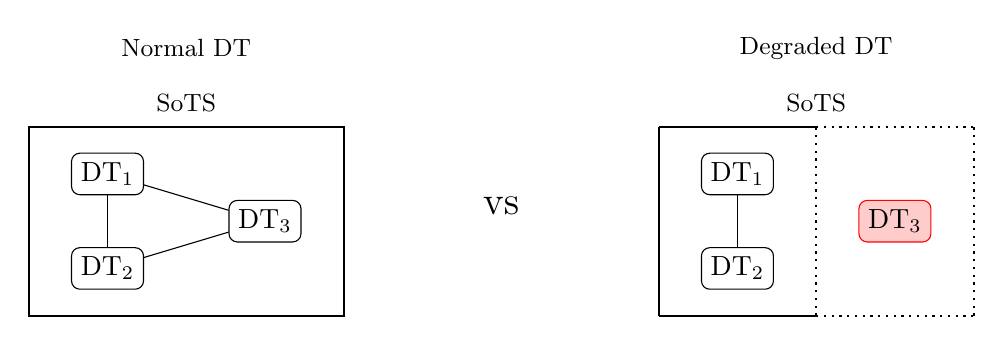
\begin{tikzpicture}[
dt/.style={draw, rounded corners=3pt, fill=white, minimum width=0.9cm}
]

% ---------- LEFT: NORMAL ----------
\node at (0,3) {\small Normal DT};

% SoTS boundary
\fill[white] (-2,-0.4) rectangle (2,2);
\draw[thick] (-2,-0.4) rectangle (2,2);
\node at (0,2.3) {\small SoTS};

% DTs
\node[dt] (dt1) at (-1,1.4) {DT$_1$};
\node[dt] (dt2) at (-1,0.2) {DT$_2$};
\node[dt] (dt3) at (1,0.8) {DT$_3$};

% connections
\draw (dt1) -- (dt2);
\draw (dt1) -- (dt3);
\draw (dt2) -- (dt3);

% ---------- VS ----------
\node at (4,1) {\Large vs};

% ---------- RIGHT: DEGRADED ----------
\node at (8,3) {\small Degraded DT};

% SoTS outer boundary
\draw[thick] (6,-0.4) -- (8,-0.4);
\draw[thick] (6,-0.4) -- (6,2);
\draw[thick] (6,2) -- (8,2);

% partition
\draw[dotted, thick] (8,-0.4) -- (8,2);

% degraded boundary
\draw[dotted, thick] (8,-0.4) -- (10,-0.4);
\draw[dotted, thick] (10,-0.4) -- (10,2);
\draw[dotted, thick] (8,2) -- (10,2);

\node at (8,2.3) {\small SoTS};

% functional active region
\fill[white] (6.1,-0.3) rectangle (7.9,1.9);

% active DTs
\node[dt] (dt1b) at (7,1.4) {DT$_1$};
\node[dt] (dt2b) at (7,0.2) {DT$_2$};

\draw (dt1b) -- (dt2b);

% degraded DT
\node[dt, draw=red, fill=red!20] (dt3b) at (9,0.8) {DT$_3$};

\end{tikzpicture}
\end{center}

\begin{center}
{\footnotesize
\tikz{\draw[red, thick, fill=red!20] (0,0) rectangle (0.25,0.25);} faulty DT}
\end{center}
\end{runningexample}

To reason about disturbances systematically, the relationships between these two dimensions must be represented in a principled way. The following section introduces a state-based model for capturing these interactions.

\section{Structured Reasoning about SoTS Reliability}\label{sec:structured-reasoning}
As discussed in \secref{sec:two-dimensional-disturbances}, disturbances in SoTS arise along two orthogonal dimensions: \emph{belonging}, which captures participation in the SoTS, and \emph{health}, which captures the operational condition of participating constituents. Although these dimensions can be considered independently, they interact during system operation. Constituents may remain present while operationally impaired, or withdraw despite remaining capable of contributing. Reliability in SoTS therefore depends both on which constituents participate and on their condition while participating. To reason about these interactions, a representation is needed that captures how constituent conditions evolve over time. State-based modelling provides such a representation by describing system behaviour in terms of discrete states and transitions between them \cite{liang2006comparative}. Each constituent can thus be understood as occupying a state defined by its participation and operational condition. \emph{I therefore model SoTS reliability using two interacting state dimensions corresponding to belonging and health}. In this model, disturbances arise from transitions between states that create conditions affecting other constituents or the system mission. Reliability can therefore be interpreted in terms of how these transitions are managed and constrained.

By explicitly representing these relationships, the model enables principled reasoning about how disturbance-causing situations emerge and how system behaviour can mitigate their effects. This perspective implies an architectural approach to reliability. Rather than requiring each constituent service to interpret participation and health changes independently, these concerns are managed through a coordination mechanism at the SoTS level. This mechanism maintains a view of constituent state and regulates participation by enforcing constraints on when and how constituents may join or withdraw based on their current condition. By preventing unreliable configurations during system operation, responsibility for managing system-level disturbances is shifted from individual services to the SoTS architecture. The following section describes how this mechanism can be formally specified and enforced.


\section{Statecharts for Modeling SoTS Reliability}
\label{sec:statecharts-reliability}

To operationalize the proposed state-based model, a formal mechanism is required to represent and enforce the interaction between belonging and health at runtime. Statecharts \cite{harel1987statecharts} provide a suitable formalism for this purpose, extending classical finite-state machines with mechanisms for modelling complex reactive behaviour. First, Statecharts support \emph{orthogonal regions}, allowing multiple state dimensions to evolve concurrently. This directly corresponds to the disturbance model, where each constituent simultaneously occupies a state in both the belonging and health dimensions. Second, Statecharts model \emph{reactive systems} whose behaviour evolves in response to events and changing system conditions \cite{harel1998modeling}, aligning naturally with SoTS environments in which constituents may join, leave, or adapt their behaviour during operation. Third, Statecharts are \emph{executable models} \cite{harel1996executable} that can be integrated into existing systems. A Statechart representation of the proposed model encodes constituent state as two orthogonal regions corresponding to belonging and health. Transitions within the Statechart regulate how constituents move between these states, enabling the system to permit, delay, or deny participation actions. In this way, Statecharts provide a concrete mechanism for enforcing participation constraints during system operation.

\subsection{State Regions for Belonging and Health}
\label{sec:constituent-state-space}

The Statechart model represents each constituent using two orthogonal state regions corresponding to the belonging and health dimensions introduced earlier. Each region contains a set of states and transitions derived from existing models in SoS lifecycle research and dependability theory.

\paragraph{Belonging}
The belonging region models the participation lifecycle of a constituent within the SoTS. It follows the SoS constituent lifecycle proposed by \citet{axelsson2019refined}, which describes the participation states a system may occupy within an SoS, as illustrated in \figref{fig:belonging-states}.

\begin{figure}[htp]
\centering
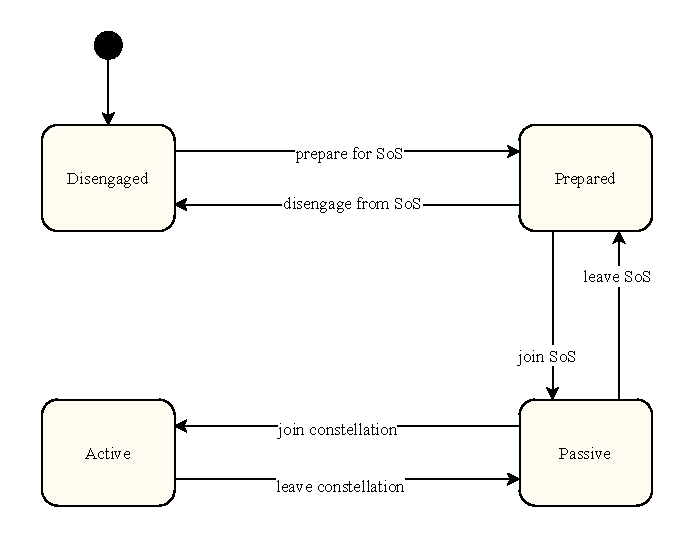
\includegraphics[width=0.55\linewidth]{figures/Approach/belonging.pdf}
\caption{Belonging Statechart}
\label{fig:belonging-states}
\end{figure}

Constituents initially reside in the \textit{Disengaged} state (referred to as \textit{Ignorant} in \citet{axelsson2019refined}), where a system possesses relevant capabilities but does not meet the requirements to participate in the SoTS. When these requirements are satisfied, the system transitions to \textit{Prepared}, indicating that it is capable of participation but has not yet joined the system. From this state, the system may \emph{join} the SoTS, entering the \textit{Passive} state where it is recognized as a constituent but not yet participating in any operational constellation. When the system becomes part of a constellation contributing to a SoTS capability, it transitions to \textit{Active}. Transitions may also occur in the opposite direction when systems leave constellations, withdraw from the SoTS, or no longer satisfy participation requirements.

\paragraph{Health}
The health region models the progressive degradation of constituent behaviour. It follows the impairment abstraction proposed by \citet{parhami1994multi-level}, which describes how impairments evolve within a system across multiple levels, as illustrated in \figref{fig:health-states}.

\begin{figure}[htp]
\centering
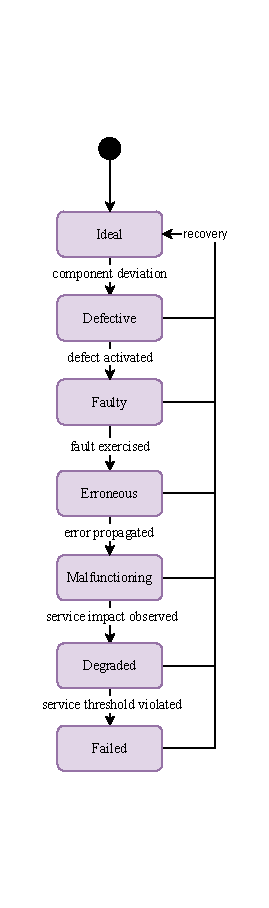
\includegraphics[
    width=0.35\linewidth,
    trim=0 2cm 0 2cm,
    clip
]{figures/Approach/health.pdf}
\caption{Health Statechart}
\label{fig:health-states}
\end{figure}

As illustrated in \figref{fig:health-states}, constituents begin in the \textit{Ideal} state, where capabilities are delivered correctly. Imperfections may introduce \textit{Defects} at the component level which, when activated, give rise to internal \textit{Faults}. If a fault contaminates system data or internal state, the system becomes \textit{Erroneous}. When these errors affect functional behaviour observable at the system level, the system transitions to the \textit{Malfunctioning} state. Continued impact on service delivery may lead to reduced capability provision, resulting in a \textit{Degraded} state, and ultimately the \textit{Failed} state where the intended capability can no longer be delivered.


\section{Reliability Levels of SoTS}\label{sec:reliability-levels}
The combination of the previously introduced statecharts defines the configurations that constituents may occupy during system operation. However, not all configurations are desirable. Certain combinations of belonging and health may destabilize ongoing activities or prevent the system from delivering its intended capabilities. Reliability in a SoTS is achieved by restricting which configurations of participation and health are permitted during operation. In the proposed architecture, these restrictions are defined and enforced through the statecharts, which constrain participation behaviour and limit the conditions under which disturbances may arise.

This perspective also allows for defining desired levels of reliability in SoTS. The following sections present four example levels---\textit{Reactive}, \textit{Proactive}, \textit{Controlled}, and \textit{Adaptive} reliability---that illustrate how reliability constraints can be expressed through the statecharts. Each level introduces additional constraints that further restrict the configurations permitted by the statecharts, reducing the potential for disturbances. These levels serve as representative examples of how SoTS reliability can be structured; other application domains may introduce additional constraints, states, or transitions depending on their operational requirements. Table~\ref{tab:reliability-levels} summarizes these levels and the mechanisms through which they are enforced.

\begin{table}[htp]
\centering
\footnotesize
\setlength{\tabcolsep}{5pt}
\begin{tabular}{p{2.2cm} p{4.5cm} p{2cm} p{4cm}}
\toprule
\textbf{Level} & \textbf{Refinement} & \textbf{Intervention Point} & \textbf{Disturbance Coverage} \\
\midrule

L1 -- Reactive 
& Joining, departure, and role changes must be announced. Participation remains uncontrolled but becomes structurally visible. 
& During/after impact 
& Improves detection of interdependency cascades \newline 
limited influence on evolution or temporary inability \\

L2 -- Proactive 
& Joining and departure are delayed through enforced notice periods, buffering structural change and reducing instability. 
& Before impact 
& Mitigates disruption from constituent evolution and temporary inability \newline
reduces cascade severity \\

L3 -- Controlled 
& Participation becomes conditional, with enforceable obligations, admission approval, and regulated withdrawal. 
& Before formation 
& Prevents unstable integration and abrupt withdrawal \newline
strongly addresses evolution-driven disturbances \\

L4 -- Adaptive 
& Responsibilities may be reassigned to preserve capability, enabling structural reconfiguration under change. 
& Before structural conditions 
& Actively compensates for structural loss \newline
mitigates interdependencies, evolution, and partial capability degradation \\

\bottomrule
\end{tabular}
\caption{Reliability Levels}
\end{table}
% ==========================================================


% \id{Reactive what? Reactive reliability? Make this more precise everywhere.}
\subsection{Level 1: Reactive Reliability}

\begin{figure}[htp]
\centering
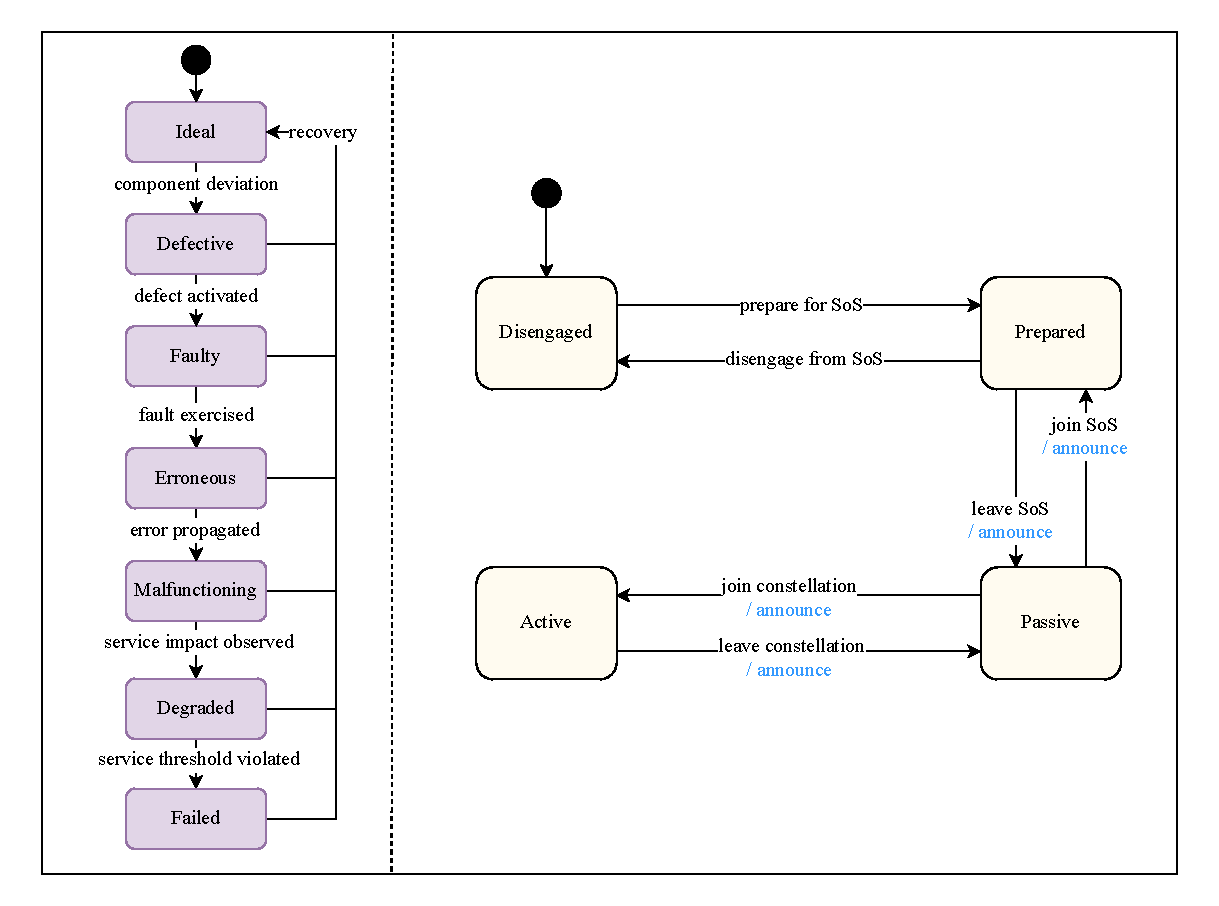
\includegraphics[width=0.9\linewidth]{figures/Approach/lv1.pdf}
\caption{Level 1: Reactive Reliability}
\label{fig:lv1}
\end{figure}

Level~1 establishes the baseline participation lifecycle for constituents in a SoTS. \citet{axelsson2019refined} observe that constituent systems must first become aware of one another in order to participate in a SoS. This awareness is represented through announcement actions on lifecycle transitions such as \textit{join SoS}, \textit{leave SoS}, \textit{join constellation}, and \textit{leave constellation}, allowing constituents to observe changes in system composition.

At this level, no constraints are imposed on the relationship between belonging and health states. Constituents may join, participate, and leave regardless of their operational condition, reflecting the loose coupling typical of open SoS environments. Disturbances are therefore handled purely reactively: participation changes are announced after they occur, but no mechanisms prevent destabilizing configurations from arising.


% ------------------------------------------------
\subsection{Level 2: Proactive Reliability}

\begin{figure}[htp]
\centering
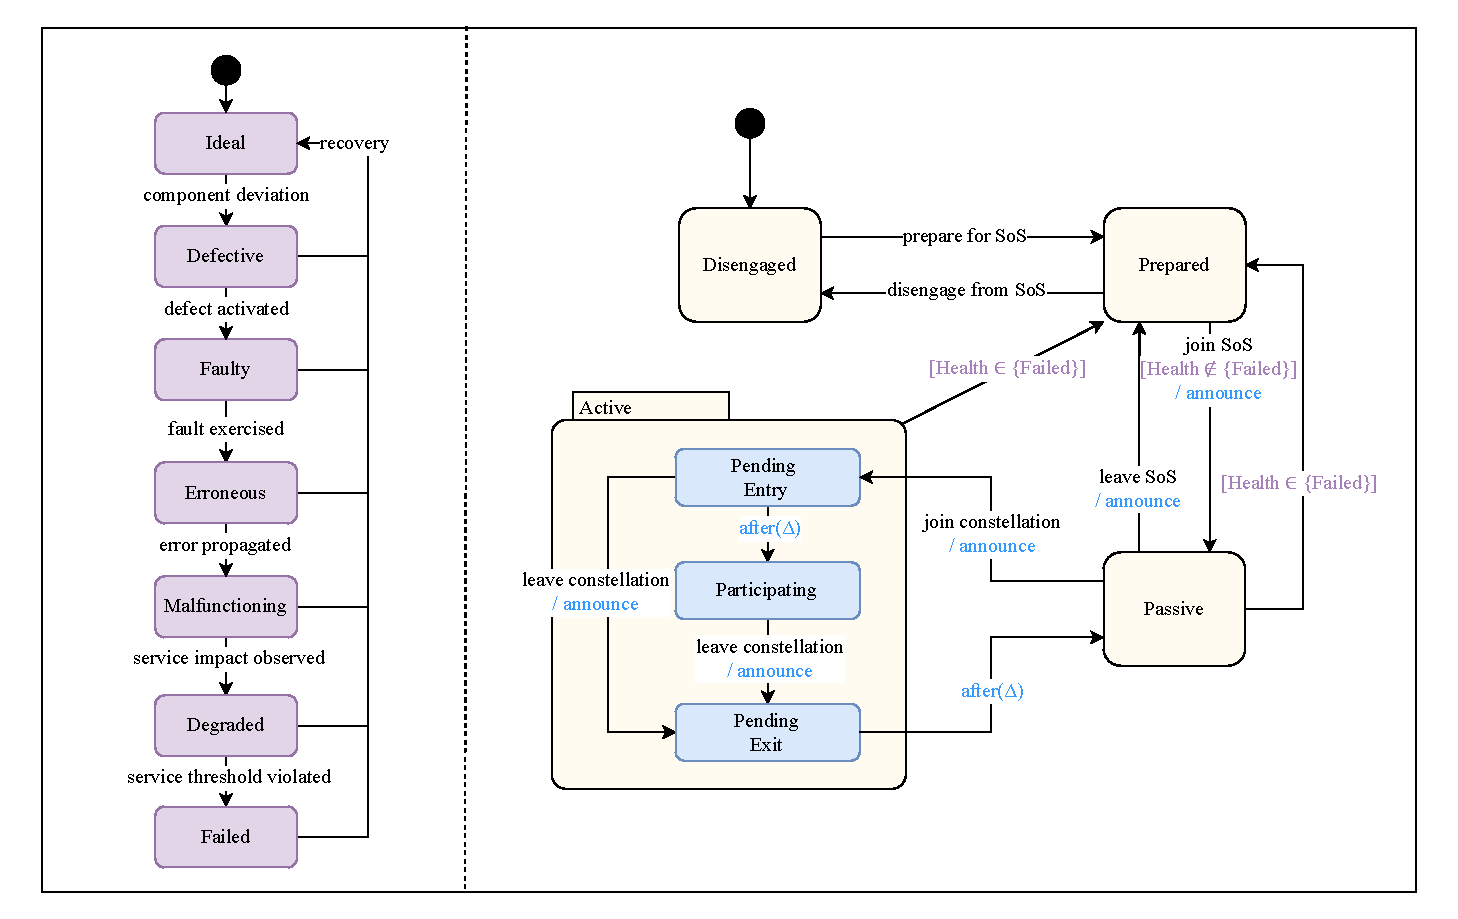
\includegraphics[width=\linewidth]{figures/Approach/lv2.pdf}
\caption{Level 2: Proactive Reliability}
\label{fig:lv2}
\end{figure}

\textit{Guarantees from Level~1 are preserved.} Level~2 introduces constraints that prevent clearly destabilizing configurations while preserving the baseline lifecycle behaviour. Participation in open SoS environments often involves dynamic entry and exit of constituents, which may disrupt ongoing activities \cite{axelsson2019refined,sage2007processes,fang2020architectural}. To address this, the \textit{Active} state is refined into three substates---\textit{Pending Entry}, \textit{Participating}, and \textit{Pending Exit}. Timed transitions (e.g., \textit{after}($\Delta$)) regulate entry and exit, introducing stabilization periods during which configuration changes can be coordinated.

In addition, constituents in the \textit{Failed} health state are prevented from joining the SoTS, and failure during participation triggers enforced withdrawal. According to \citet{parhami1994multi-level}, a failed constituent can no longer deliver the required service, making participation inconsistent with this condition.

These refinements remove configurations in which a constituent remains in a participating state despite being unable to contribute its required capability. Disturbances are therefore mitigated by preventing failed constituents from joining and by introducing stabilization periods that allow the system to prepare for participation changes.
% ------------------------------------------------

\subsection{Level 3: Controlled Reliability}

\begin{figure}[htp]
\centering
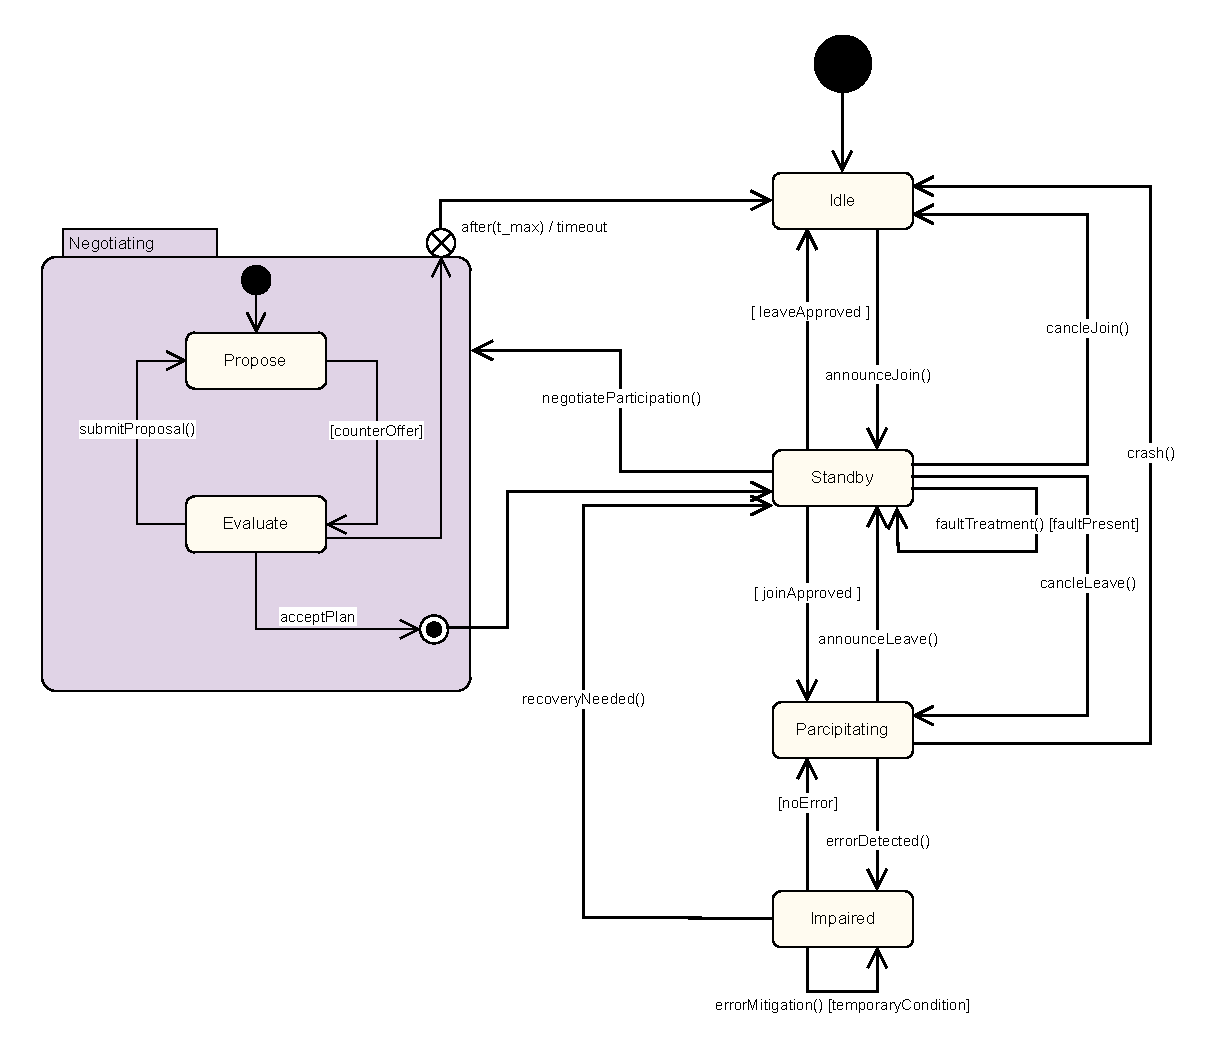
\includegraphics[width=\linewidth]{figures/Approach/lv3.pdf}
\caption{Level 3: Controlled Reliability}
\label{fig:lv3}
\end{figure}

\textit{Guarantees from Level~2 are preserved.} Level~3 further restricts participation by introducing coordination mechanisms that regulate admission and withdrawal of constituents. SoS coordination frequently involves negotiation between participating systems \cite{axelsson2019refined,fisher2006emergent,damm2015conceptual}. To represent this process, the \textit{Passive} state is refined into two substates: \textit{Available} and \textit{Negotiating}. Constituents may issue \textit{join requests} when operating under favourable conditions, while constellations may issue \textit{join invitations} when additional capabilities are required. Withdrawal behaviour is also constrained through the introduction of the \textit{exitDenied} transition, which prevents constituents from leaving while active commitments or agreements require their continued participation.

Together, these mechanisms ensure that admission to the \textit{Active} state occurs through coordinated negotiation rather than uncontrolled entry, and that withdrawal cannot occur arbitrarily. Disturbances are therefore mitigated by preventing unstable collaborations from forming and by avoiding disruption caused by spontaneous withdrawal.
% ------------------------------------------------
\subsection{Level 4: Adaptive Reliability}\label{sec:lv4}

\begin{figure}[htp]
\centering
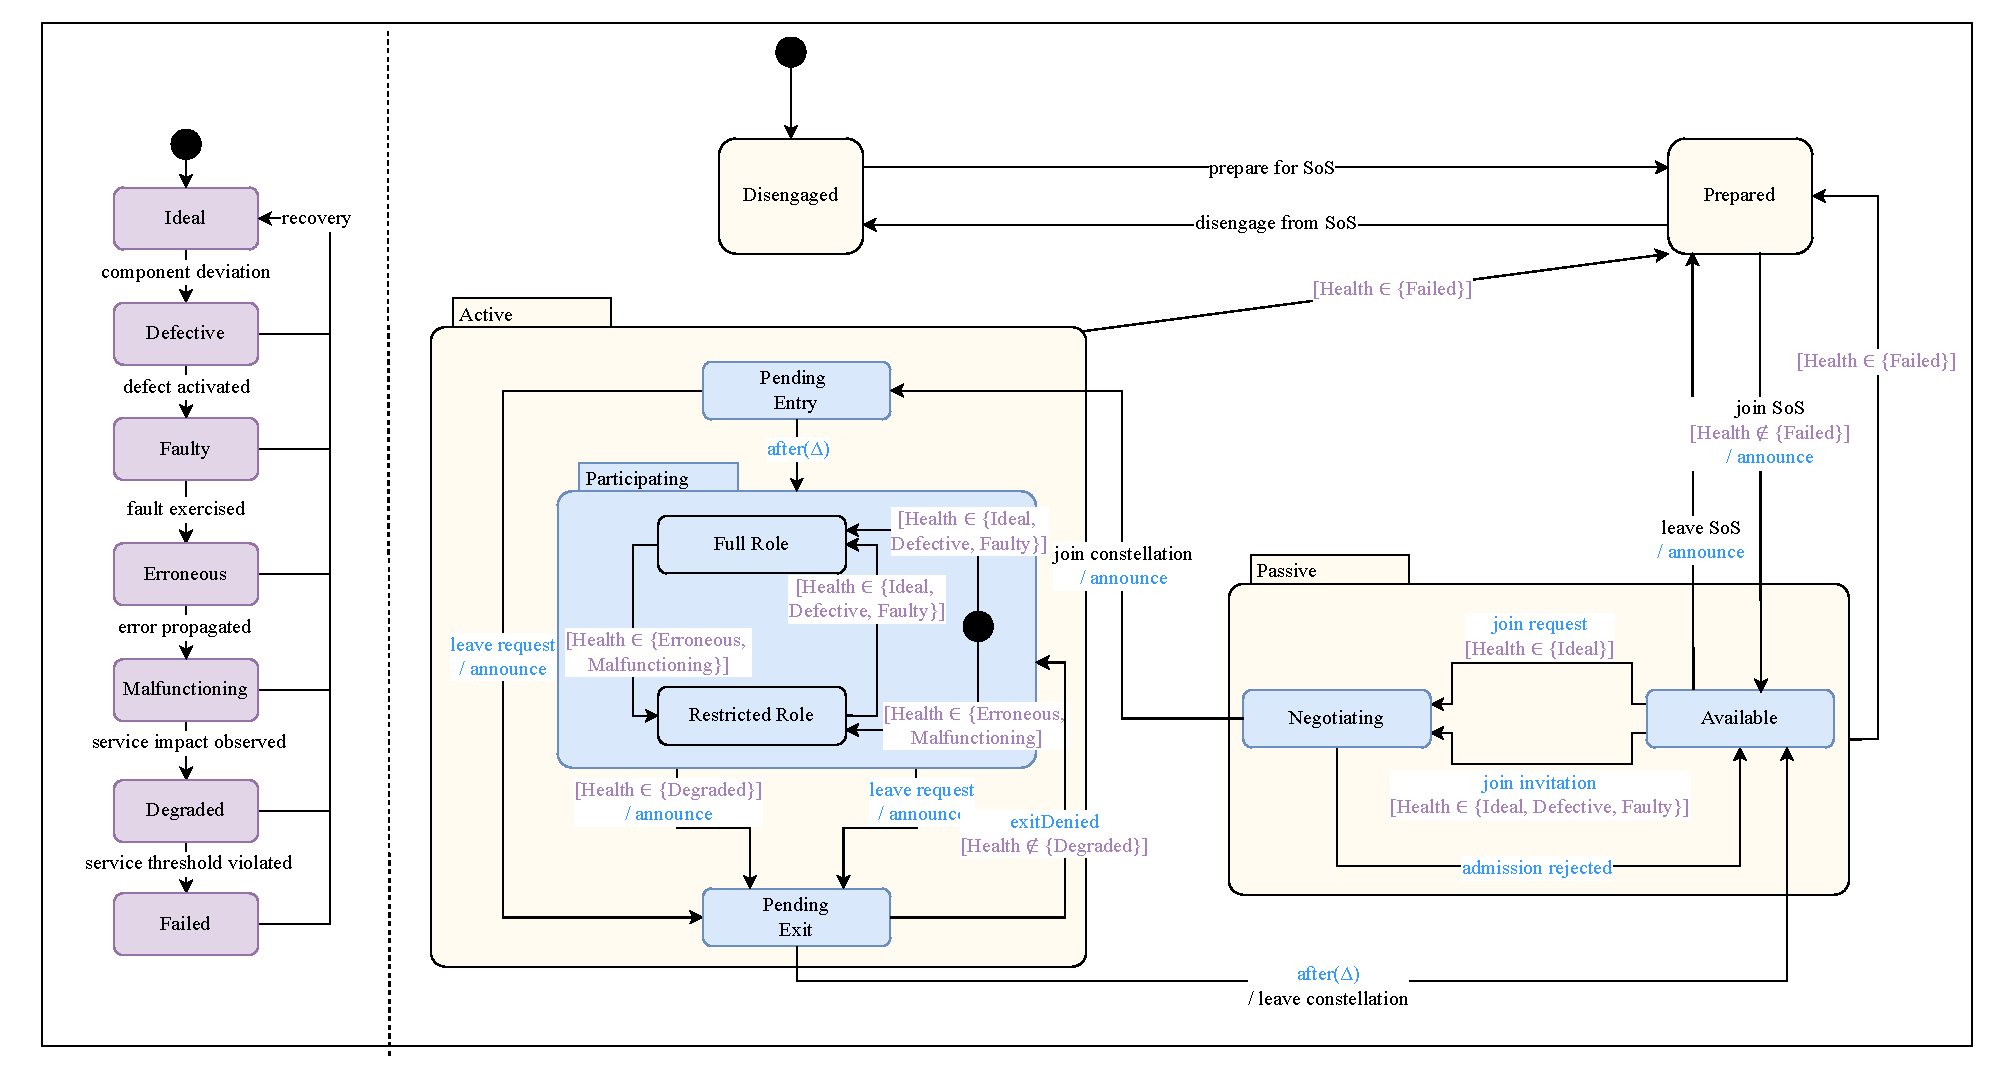
\includegraphics[width=\linewidth]{figures/Approach/lv4.pdf}
\caption{Level 4: Adaptive Reliability}
\label{fig:lv4}
\end{figure}

\textit{Guarantees from Level~3 are preserved.} Level~4 introduces adaptive behaviour based on the operational health of participating constituents. To support this adaptation, the \textit{Participating} state is refined into two substates: \textit{Full Role} and \textit{Restricted Role}. Health-based transitions allow impaired constituents to reduce their influence on system behaviour by moving to restricted participation roles. Additionally, when compensation is insufficient to reduce uncertainty to acceptable levels, withdrawal from the \textit{Restricted Role} is enforced to prevent unreliable participation. When degradation progresses further, \textit{leave request} transitions enforce controlled withdrawal before complete failure occurs. These mechanisms ensure that deteriorating constituents either operate in a limited role or exit the system before their condition can destabilize ongoing activities.

Disturbances are therefore mitigated through adaptive containment, where impaired constituents are progressively constrained as their health deteriorates. Constituents may transition from a \textit{Full Role} to a \textit{Restricted Role}, reducing their influence on system behaviour while compensation mechanisms address missing or degraded capabilities. If deterioration continues, enforced exit transitions remove the constituent before complete failure can introduce destabilizing behaviour or incorrect outputs.



\section{Fault Tolerance through SoTS Reliability}
\label{sec:reducing-fault-tolerance-burden}

Disturbances in SoTS cannot be completely eliminated due to their inherent complexity and dynamic nature \cite{nielsen2015systems,ferreira2023towards}. As a result, fault-tolerance mechanisms remain essential for detecting and managing faults during system execution \cite{hanmer2013patterns,avizienis2004basic}. These mechanisms typically operate across multiple layers, including individual constituent services and the SoTS coordination layer.

Conventional fault-tolerance approaches, developed in SoS and applied in SoTS, include redundancy, monitoring, reallocation, predictive estimation, state persistence, fallback behaviour, and asynchronous communication \cite{ferreira2021reliability,uday2015designing,abdelmoumen2026comprehensive,esterle2021digital,larsen2024towards,lopez2023modeling,chen2018digital,joseph2021aggregated}. In most implementations, these mechanisms are embedded within individual services, requiring each service to handle disturbances arising both from internal faults and from system-level dynamics such as the participation and operational condition of other constituents.

The reliability model proposed in this chapter shifts part of this responsibility to the architectural level. By explicitly managing the belonging and health states of constituents, the SoTS layer constrains which state combinations and transitions are permitted during operation. This reduces the number of disturbance scenarios that individual services must handle, allowing them to focus on faults specific to their own functionality rather than the broader system-level dynamics.

\begin{runningexample}{CEP-Based SoTS}
In a traditional design, a CEP service may encounter partial or inconsistent event streams when a DT fails or leaves the system. In the proposed architecture, the SoTS coordination layer monitors constituent states and can reassign responsibilities, estimate missing observations, or restrict decisions to reliable participants. This management of participation and health at the architectural level allows the CEP service to concentrate on service-specific fault tolerance, such as retrying event delivery, buffering delayed events, or recovering from internal processing errors.
\end{runningexample}

By separating responsibilities in this way, the architecture clarifies the roles of different system layers: SoTS engineers manage participation and operational reliability at the architectural level, while service developers handle service-level fault tolerance. Reliability in SoTS therefore emerges from a layered combination of SoTS-level coordination and service-level mechanisms, providing a more robust and manageable approach to complex system dynamics.


\section{Mapping Reliability Levels to SoTS Types}\label{sec:reliability-compatibility}
\begin{table}[htp]
\centering
\footnotesize
\begin{tabular}{p{1.7cm} c c c c c c}
\toprule
\textbf{Reliability Level} 
& \textbf{Directed} 
& \textbf{Acknowledged} 
& \textbf{Collaborative} 
& \textbf{Virtual} 
& \textbf{Spec. DT}
& \textbf{Spec. DT + PT} \\
\midrule

Reactive     & X & X & X & X & X & X \\
Proactive    & X & X & X &   & X & X \\
Controlled   & X & X &   &   & X & X \\
Adaptive     & X &   &   &   & X & X \\

\bottomrule
\end{tabular}
\caption{Compatibility of reliability levels with SoTS types}
\end{table}
The reliability levels defined in this chapter impose progressively stronger constraints on constituent participation and behaviour. Higher levels govern how systems join, participate in, and withdraw from coordinated activities. The feasibility of enforcing these constraints depends on the degree of coordination authority available within the SoTS architecture. SoTS architectures can be broadly classified as directed, acknowledged, collaborative, or virtual, differing primarily in how strongly constituent behaviour can be coordinated \secref{sec:literature-review-classification}.

Directed SoTS feature centralized coordination mechanisms, enabling direct enforcement of behavioural constraints. Several implementations describe DT ecosystems coordinated through hierarchical orchestration platforms controlled by a system-level DT that aggregates system information and supports centralized decision-making \cite{novak2022digitalized,parri2021framework,reiche2021digital,dickopf2019holistic}. In these architectures, all reliability constraints are technically enforceable, as participation and operational conditions can be monitored and controlled centrally. Acknowledged SoTS retain a coordinating authority but allow constituents to pursue partially independent objectives. Platforms integrating multiple DTs while permitting semi-independent operation are common examples \cite{parri2019jarvis,maheshwari2022digital,bellavista2023requirements,binder2021utilizing}. Here, many reliability constraints remain enforceable, though coordination relies more on negotiation or policy agreements among participants. Collaborative and virtual SoTS, in contrast, depend primarily on voluntary participation and decentralized interaction. Behaviour is determined locally by individual systems, and runtime composition of DTs occurs without centralized control \cite{acharya2023twins,gil2023modeling,esterle2021digital}. In such environments, enforcing system-wide reliability constraints is significantly more challenging. \tabref{tab:sots-reliability-compatibility} summarizes how these architectural differences affect the feasibility of enforcing reliability constraints across SoTS types.